\label{s:hz}
\subsection{Potentially Rocky Planets in the Habitable Zone}
In order for this catalog to be used to understand the occurrence of rocky exoplanets in the habitable zone of a sun-like stars, it needs to identify small, temperate candidates around G-dwarf stars.  In this section we highlight those candidates in that part of the DR25 KOI catalog and mention some of the issues related to using this catalog to calculate occurrence rates.

The DR25 catalog uses the transit depth and the period, along with the DR25 stellar table \citet{Mathur2017ApJS}, to derive the planet radius and the semi-major axis of the planet's orbit.  From these we calculate the insolation flux relative to the insolation flux of the earth:

\begin{equation}
S_{p} = \frac{R_{p}^{2} \cdot (T_{\star}/5777)^{4}}{a^{2}}
\end{equation}

\noindent where $a$ is the semi-major axis of the planet's orbit in AU, \tstar{} is in Kelvin, 5777~K is the effective temperature of the Sun, and \sp{} and \rp{} are in Earth units. The errors for both insolation flux and radii include the errors from the DR25 stellar table. See Figure~\ref{f:hzPlot} for a plot of planet radius against insolation flux at the small, cool end of the DR25 catalog. On this figure the color indicates the stellar temperature and the size of the point indicates the disposition score.  Notice that this part of the catalog is dominated by K and M stars despite the fact that the exoplanet search targets G stars \citet{Batalha2010}.

\begin{figure*}
    \centering
    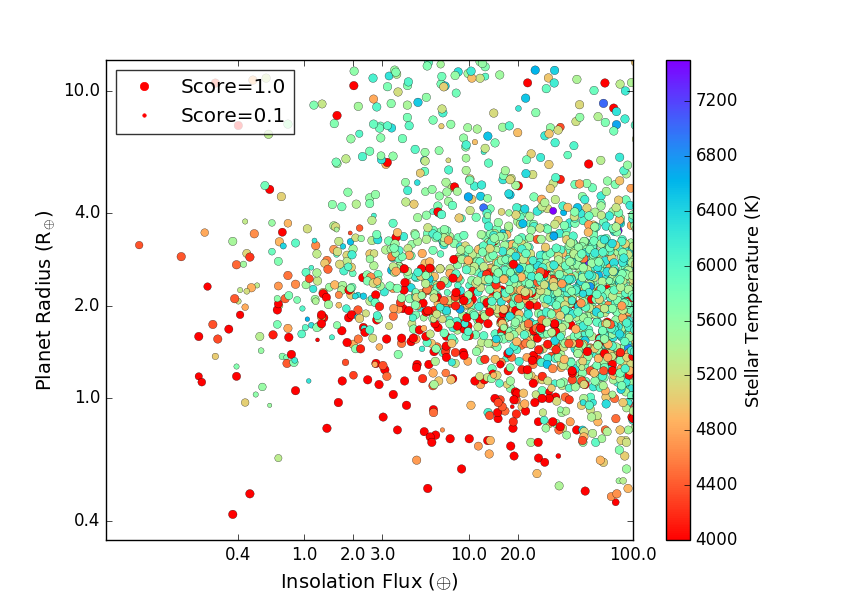
\includegraphics[width=1.1\linewidth]{fig-CatalogRadiusInsolScore.png}
    \caption{DR25 Exoplanet Candidates plotted as planet radius against Insolation Flux, in units of the flux that the Earth recieves from the Sun. The stellar temperature is given by the color of the circle and the size of the circle indicates the Disposition Score. The planet radii are derived from the MCMC fits. }
    \label{f:hzPlot}
\end{figure*}

In Table~\ref{t:hz} we highlight the DR25 catalog candidates that are potentially terrestrial and fall in or near the habitable zone of their star.  We select these stars to be any candidate with 1) a disposition score above 0.5, 2)  one sigma error bars that indicate the radius could be smaller than 1.8 \rearth, and 3) one sigma error bars in insolation flux that place them in the optimistic habitable zone defined by \citet{Kopparapu2013} (i.e. the inner edge is the runaway greenhouse for Venus and the outer edge is given by early Mars [NEED A BETTER DESCRIPTION]). Any candidate whose error in radii or insolation flux is larger than 200 per cent have been eliminated because this usually indicates a poor fit.  This produces 44 candidates in the DR25 catalog. Of these, 10 are new to the DR25 catalog, which is in indicated in Table~\ref{t:hz} by a star.
A manual review of these new candidates indicate they all are low signal to noise and 
 

The reliability measurements for this catalog indicate that the false alarm reliabiltiy  disposition score cut of 0.5 yields a false alarm reliability of $\appro$80 per cent for those with periods from 200--500 \,d.  

We inspected each of these new ones by hand. They are all low signal to noise and we cannot absolutely rule out any as a being caused entirely by noise, however our metrics indicate

In Figure~\ref{f:hzNarrow} we plot those candidates